% !TeX root = max_formula.tex
\documentclass[a4paper,11pt]{jsarticle}

% 英文化
\usepackage[english]{babel}
% 数式
\usepackage{amsmath}
\usepackage{amsfonts}
\usepackage{amsthm}
\usepackage{amssymb}
\usepackage{bm}
\usepackage{mathtools}
% 画像
\usepackage[dvipdfmx]{graphicx}
% 箇条書き
\usepackage{enumitem}

% 枠付き文章
\usepackage{ascmac}

\newcommand{\MiniBox}[1]{\fbox{
  \begin{minipage}{.8\textwidth}
    #1
  \end{minipage}
}}

\SetLabelAlign{Center}{\hfil#1\hfil}
\SetLabelAlign{CenterWithParen}{\hfil(\makebox[1.0em]{#1})\hfil}

\newtheorem{thm}{Theorem}[section]
\newtheorem{prop}[thm]{Proposition}
\newtheorem{lem}[thm]{Lemma}
\newtheorem{cor}[thm]{Corollary}
\newtheorem{conj}[thm]{Conjecture}
\theoremstyle{definition}
\newtheorem{dfn}[thm]{Definition}
\newtheorem{rem}[thm]{Remark}
\newtheorem{fact}[thm]{Fact}


% Mathematical Sets
\newcommand{\NaturalNumberSet}{\mathbb{N}}
\newcommand{\RealNumberSet}{\mathbb{R}}
\newcommand{\NDemenstionalRealEuclideanSpace}{\mathbb{R}^n}
\newcommand{\MDemenstionalRealEuclideanSpace}{\mathbb{R}^m}
\newcommand{\NDemenstionalRealSymmetricMatrixSpace}{\mathbb{S}^n}
\newcommand{\NDemenstionalRealOthonormalMatrixSpace}{\mathcal{U}_n}


% Symbols like prefix
\newcommand{\Closure}[1]{\text{\rm cl\:${#1}$}} % cl
\newcommand{\Interior}[1]{\text{\rm int\:${#1}$}} % int
\newcommand{\Domain}[1]{\text{\rm dom\:${#1}$}} % dom
\newcommand{\Epigraph}[1]{\text{\rm epi\:${#1}$}} % epi
\newcommand{\KEpigraph}[1]{\text{\rm epi$_K$\:${#1}$}} % epi_K
\newcommand{\LevelSets}[2]{\text{\rm lev\:$({#1}, {#2})$}} % lev
\newcommand{\Trace}[1]{\text{\rm tr$({#1})$}} % tr
\newcommand{\Diagnosis}[1]{\text{\rm diag\:${#1}$}} % diag
\newcommand{\InnerProduct}[2]{\left\langle {#1},{#2}\right\rangle} % <x,y>
\newcommand{\Norm}[1]{\left\lVert {#1} \right\rVert} % ||x||

% Extended real valued function e.g. f: X -> Rv{+∞}
% #1: function symbol
% #2: domain of function
\newcommand{\ExtendedRealValuedFunction}[2]{{#1}: {#2} \to \RealNumberSet \cup \{+\infty\}}
\newcommand{\VectorValuedFunction}[3]{{#1}\:\colon{#2} \to {#3}}


% Conjugate function e.g. f*
% #1: function symbol
\newcommand{\ConjugateFunction}[1]{{#1}^*}

% Support function e.g. f*
% #1: set symbol
\newcommand{\SupportFunction}[1]{\sigma_{#1}}

% Indicator function e.g. f*
% #1: set symbol
\newcommand{\IndicatorFunction}[1]{\delta_{#1}}

% (Useful) Texts
\newcommand{\SuchThat}{\:\text{\rm s.t.}\:}

% Set form e.g. {x | ...}
% #1: element
% #2: conditions
\newcommand{\SetForm}[2]{
  \{{#1}\:|\:{#2}\}
}

\begin{document}

\title{%
  A Generalized Definition of Asymptotic Functions \\
  for Vector-Valued Functions}
\author{Ryota Iwamoto}
\date{\today}
\maketitle

目標: ベクトル値関数に対する漸近関数の定義を与える. 特に、拡張実数値関数における proper, l.s.c., convex な関数の
漸近関数の性質を保持するように定義する。

背景: ベクトル値関数の最適化問題において, 漸近関数は有用である. また、\cite[F. Flores-Baz\'{a}n, R. L\'{o}pez and C. Vera (2024)]{Flores2024} において, ベクトル値関数に対する漸近関数の定義が与えられている.
しかし、その定義は一般的なものではなく、各成分に対して拡張実数値関数が与えられている場合のものに限る. そこで、本研究では、一般のベクトル値関数に対する漸近関数の定義を与える.

応用: ベクトル値関数に対する漸近関数の定義を与えることで、\cite[A.Auslender (1999)]{Auslender99} 内で述べられている Composite model 
\begin{equation}
  \inf_{x \in \mathbb{R}^n} f_0(x) + p(F(x))
\end{equation}
における最適化問題に対して、ベクトル値関数の漸近関数を適用することができる.

\section{Basic Definitions}

以下は拡張実数値関数に対する漸近関数の定義と主な性質である.

\begin{dfn}[\mbox{\cite[p.48 Def 2.5.1]{Auslender03}}]
  For any proper function $\ExtendedRealValuedFunction{f}{\NDemenstionalRealEuclideanSpace}$, there exists a unique function $\ExtendedRealValuedFunction{f_{\infty}}{\NDemenstionalRealEuclideanSpace}$ associated with $f$, called the asymptotic function, such that $\Epigraph{f_\infty} = (\Epigraph{f})_{\infty}$.
\end{dfn}

\begin{prop}[\mbox{\cite[p.50 Prop 2.5.2]{Auslender03}}]
  Let $\ExtendedRealValuedFunction{f}{\NDemenstionalRealEuclideanSpace}$ be a proper, l.s.c, convex function. The asymptotic function $f_{\infty}$ is positively homogeneous, l.s.c., proper convex function, and for any $d \in \NDemenstionalRealEuclideanSpace$, one has
  \begin{equation}
    f_{\infty}(d) = \sup \{f(x+d) -f(x) \:|\: x \in \Domain{f}\}
  \end{equation}
  and
  \begin{equation}
    f_{\infty}(d) = \lim_{t \to +\infty} \frac{f(x+td) -f(x)}{t} = \sup_{t>0} \frac{f(x+td) - f(x)}{t}, \forall x \in \Domain{f}.
  \end{equation}
\end{prop}

ベクトル値関数における proper の性質は以下のように定義される.\\
\par
\MiniBox{
  There are notions given for functions with extended real values that can be formulated also 
  for functions mapping from X into vector spaces.
  Let $V$ be Hausdorff locally convex space partially ordered 
  by the convex cone $K$ and $\bar{V}=V \cup \{\pm \infty_K\} $.

  The domain of a vector function $\VectorValuedFunction{h}{X}{\bar{V}}$ is the set 
  $\Domain{h} \coloneqq \SetForm{x \in X}{h(x) \ne +\infty_K}$. When $h(x) \ne -\infty_K$ for all $x \in X$ and 
  $\Domain{h} \ne \emptyset$ we call $h$ proper. $K$-epigraph of a vector function 
  $\VectorValuedFunction{h}{X}{\bar{V}}$ is the set $\KEpigraph{h} \coloneqq \SetForm{(x,v) \in X \times V}{h(x) \leq_K v}$.

  [Duality in Vector Optimization p.22]
}\\
\par
また、ベクトル値関数における lower semicontinuous の性質は以下のように考えられる.\\
\par
\MiniBox{
  There are several extensions of the notion of lower semicontinuity for vector functions based on the properties 
  of the lower semicontinuous functions. We recall here three of them, 
  which are mostly used in convex optimization. 
  Like before, $V$ is a Hausdorff locally convex space partially ordered by the convex cone $K$.

  [Duality in Vector Optimization p.29]
}\\
\par
\begin{dfn}[\mbox{\cite[p.29 Def 2.2.13]{Bot2009}}]
  A function $\VectorValuedFunction{h}{X}{V\cup\{+\infty_K\}}$ is called
  \begin{enumerate}
    \item $K$-lower semicontinuity at $x \in X$ if for any neighborhood $W$ of zero in $V$ 
    and for any $b \in V$ satisfying $b \leq_K h(x)$, there exists a neighborhood $U$ of $x$ in $X$ 
    such that $h(U) \subset b + W + K \cup \{+\infty_K\}$.
    \item star $K$-lower semicontinuous at $x \in X$ if $(k^*h)$ is lower semicontinuous at $x$ for all $k^* \in K^*$.
  \end{enumerate}
\end{dfn}

Now, when $K$ is a cone in $X$, its topological dual cone, further called simply dual cone, is 
\begin{equation}
  K^* = \SetForm{x^* \in X^*}{\InnerProduct{x^*}{x} \geq 0, \forall x \in K}.
\end{equation}

\begin{conj}
  Let $\VectorValuedFunction{f}{\NDemenstionalRealEuclideanSpace}{\MDemenstionalRealEuclideanSpace}$ be a vector-valued function. 
  Then, 
  \begin{flalign}
    &\forall x \in \NDemenstionalRealEuclideanSpace,\: \exists! y \in \MDemenstionalRealEuclideanSpace \:\text{and}\: K(x) \subset \MDemenstionalRealEuclideanSpace \SuchThat\quad \notag &
  \end{flalign}
  \begin{align}
    (\KEpigraph{f})_{\infty} \cap (\{x\}\times\MDemenstionalRealEuclideanSpace) = (x, y) + (\{0\} \times K(x))
  \end{align}
  and
  \begin{equation}
    K(x) \text{ is a cone in } \MDemenstionalRealEuclideanSpace \quad\text{and}\quad k(x) \supset K.
  \end{equation}
\end{conj}

\begin{conj}
  Let $\VectorValuedFunction{f}{\NDemenstionalRealEuclideanSpace}{\MDemenstionalRealEuclideanSpace}$ be a vector-valued function 
  and $K$ be a closed convex cone in $\MDemenstionalRealEuclideanSpace$. Then, 
  \begin{equation}
    \exists! d \in \MDemenstionalRealEuclideanSpace \SuchThat (\bigcup_{x \in \NDemenstionalRealEuclideanSpace} (f(x) + K))_{\infty} = \text{cone\:}\{d\} + K.
  \end{equation}
\end{conj}

\begin{conj}
   Let $a, b \in \MDemenstionalRealEuclideanSpace$ and $K$ be a closed convex pointed cone in $\MDemenstionalRealEuclideanSpace$ where $\Interior{K} \ne \emptyset$. 
   Then, the following statements hold:
   \begin{enumerate}
    \item $(a + K) \cap (b + K) \ne \emptyset$;
    \item $(a + K) \subset (b + K) \Rightarrow (a + K) \cap (b + K) = a + K$;
    \item $(a + K) \nsubseteq (b + K) \Rightarrow (a + K) \cap (b + K) = (a + b) + K$.
   \end{enumerate}
\end{conj}

\begin{lem}
  Let $a$ be a vector in $\NDemenstionalRealEuclideanSpace$ and $K$ be a closed convex cone in $\NDemenstionalRealEuclideanSpace$ where $\Interior{K} \ne \emptyset$. 
  Then, $(a + K)_{\infty} = K$.
\end{lem}

\begin{proof}
  Since $K$ is a cone, $0 \in K$. As a result, one has $a \in a + K$. By the consequence of Auslender's statement (p.29), it holds that
  \begin{equation}
    C_{\infty} = \bigcap_{t > 0} \frac{C - x}{t}, \forall x \in C. \notag
  \end{equation}
  Thus, we obtain 
  \begin{equation}
    (a + K)_{\infty} = \bigcap_{t > 0} \frac{(a + K) - a}{t} = \bigcap_{t > 0} \frac{K}{t} = K. \notag
  \end{equation}
\end{proof}

\begin{rem}
  実数値関数の漸近関数は、漸近方向での単位ベクトルあたりの値の変換を表している。その性質をベクトル値関数に応用させると
  『漸近方向での単位ベクトルあたりのベクトルの変化』を表すことになる。ベクトルの変化とは、ベクトルの向きと大きさの変化を表す。
  ベクトルの大きさの増加が2乗比例のような場合には漸近関数の値を $\infty_{K}$ とすると良い。一方で、漸近方向が有界、もしくはベクトルの大きさの変化が減少
  している場合には、漸近関数の値を $0$ とすると良い。
\end{rem}

\begin{dfn}\label{dfn1:asymptotic_function}
  Let $\VectorValuedFunction{f}{\NDemenstionalRealEuclideanSpace}{\MDemenstionalRealEuclideanSpace}$ be a vector-valued function 
  and $K$ be a closed convex cone in $\MDemenstionalRealEuclideanSpace$. Then, the asymptotic function of $f$ to $d \in \NDemenstionalRealEuclideanSpace, ||d|| = 1$ is defined as
  \begin{equation}
    f_{\infty}(td) = k(t) a, k(t) \coloneqq b_0 t : \text{ratio}, a \in (\cup_{x \in \NDemenstionalRealEuclideanSpace} \{f(x)\})_{\infty}, ||a|| = 1.
  \end{equation}
\end{dfn}

\begin{rem}
  $\cup_{x \in \NDemenstionalRealEuclideanSpace} \{f(x)\} = \text{img} f$ に対して漸近錐 $(\cup_{x \in \NDemenstionalRealEuclideanSpace} \{f(x)\})_{\infty}$ 
  が与えられた順序錐 $K$ に含まれるかどうかが重要である。なぜなら、それが順序錐に含まれない場合、漸近錐の要素同士を比較することができないから
  である。順序が定まらないということは、その方向に関してベクトルが増加しているかがわからないことを意味する。
\end{rem}

\centering
\begin{figure}[h]
  \centering
  \begin{minipage}[b]{0.49\columnwidth}
      \centering
      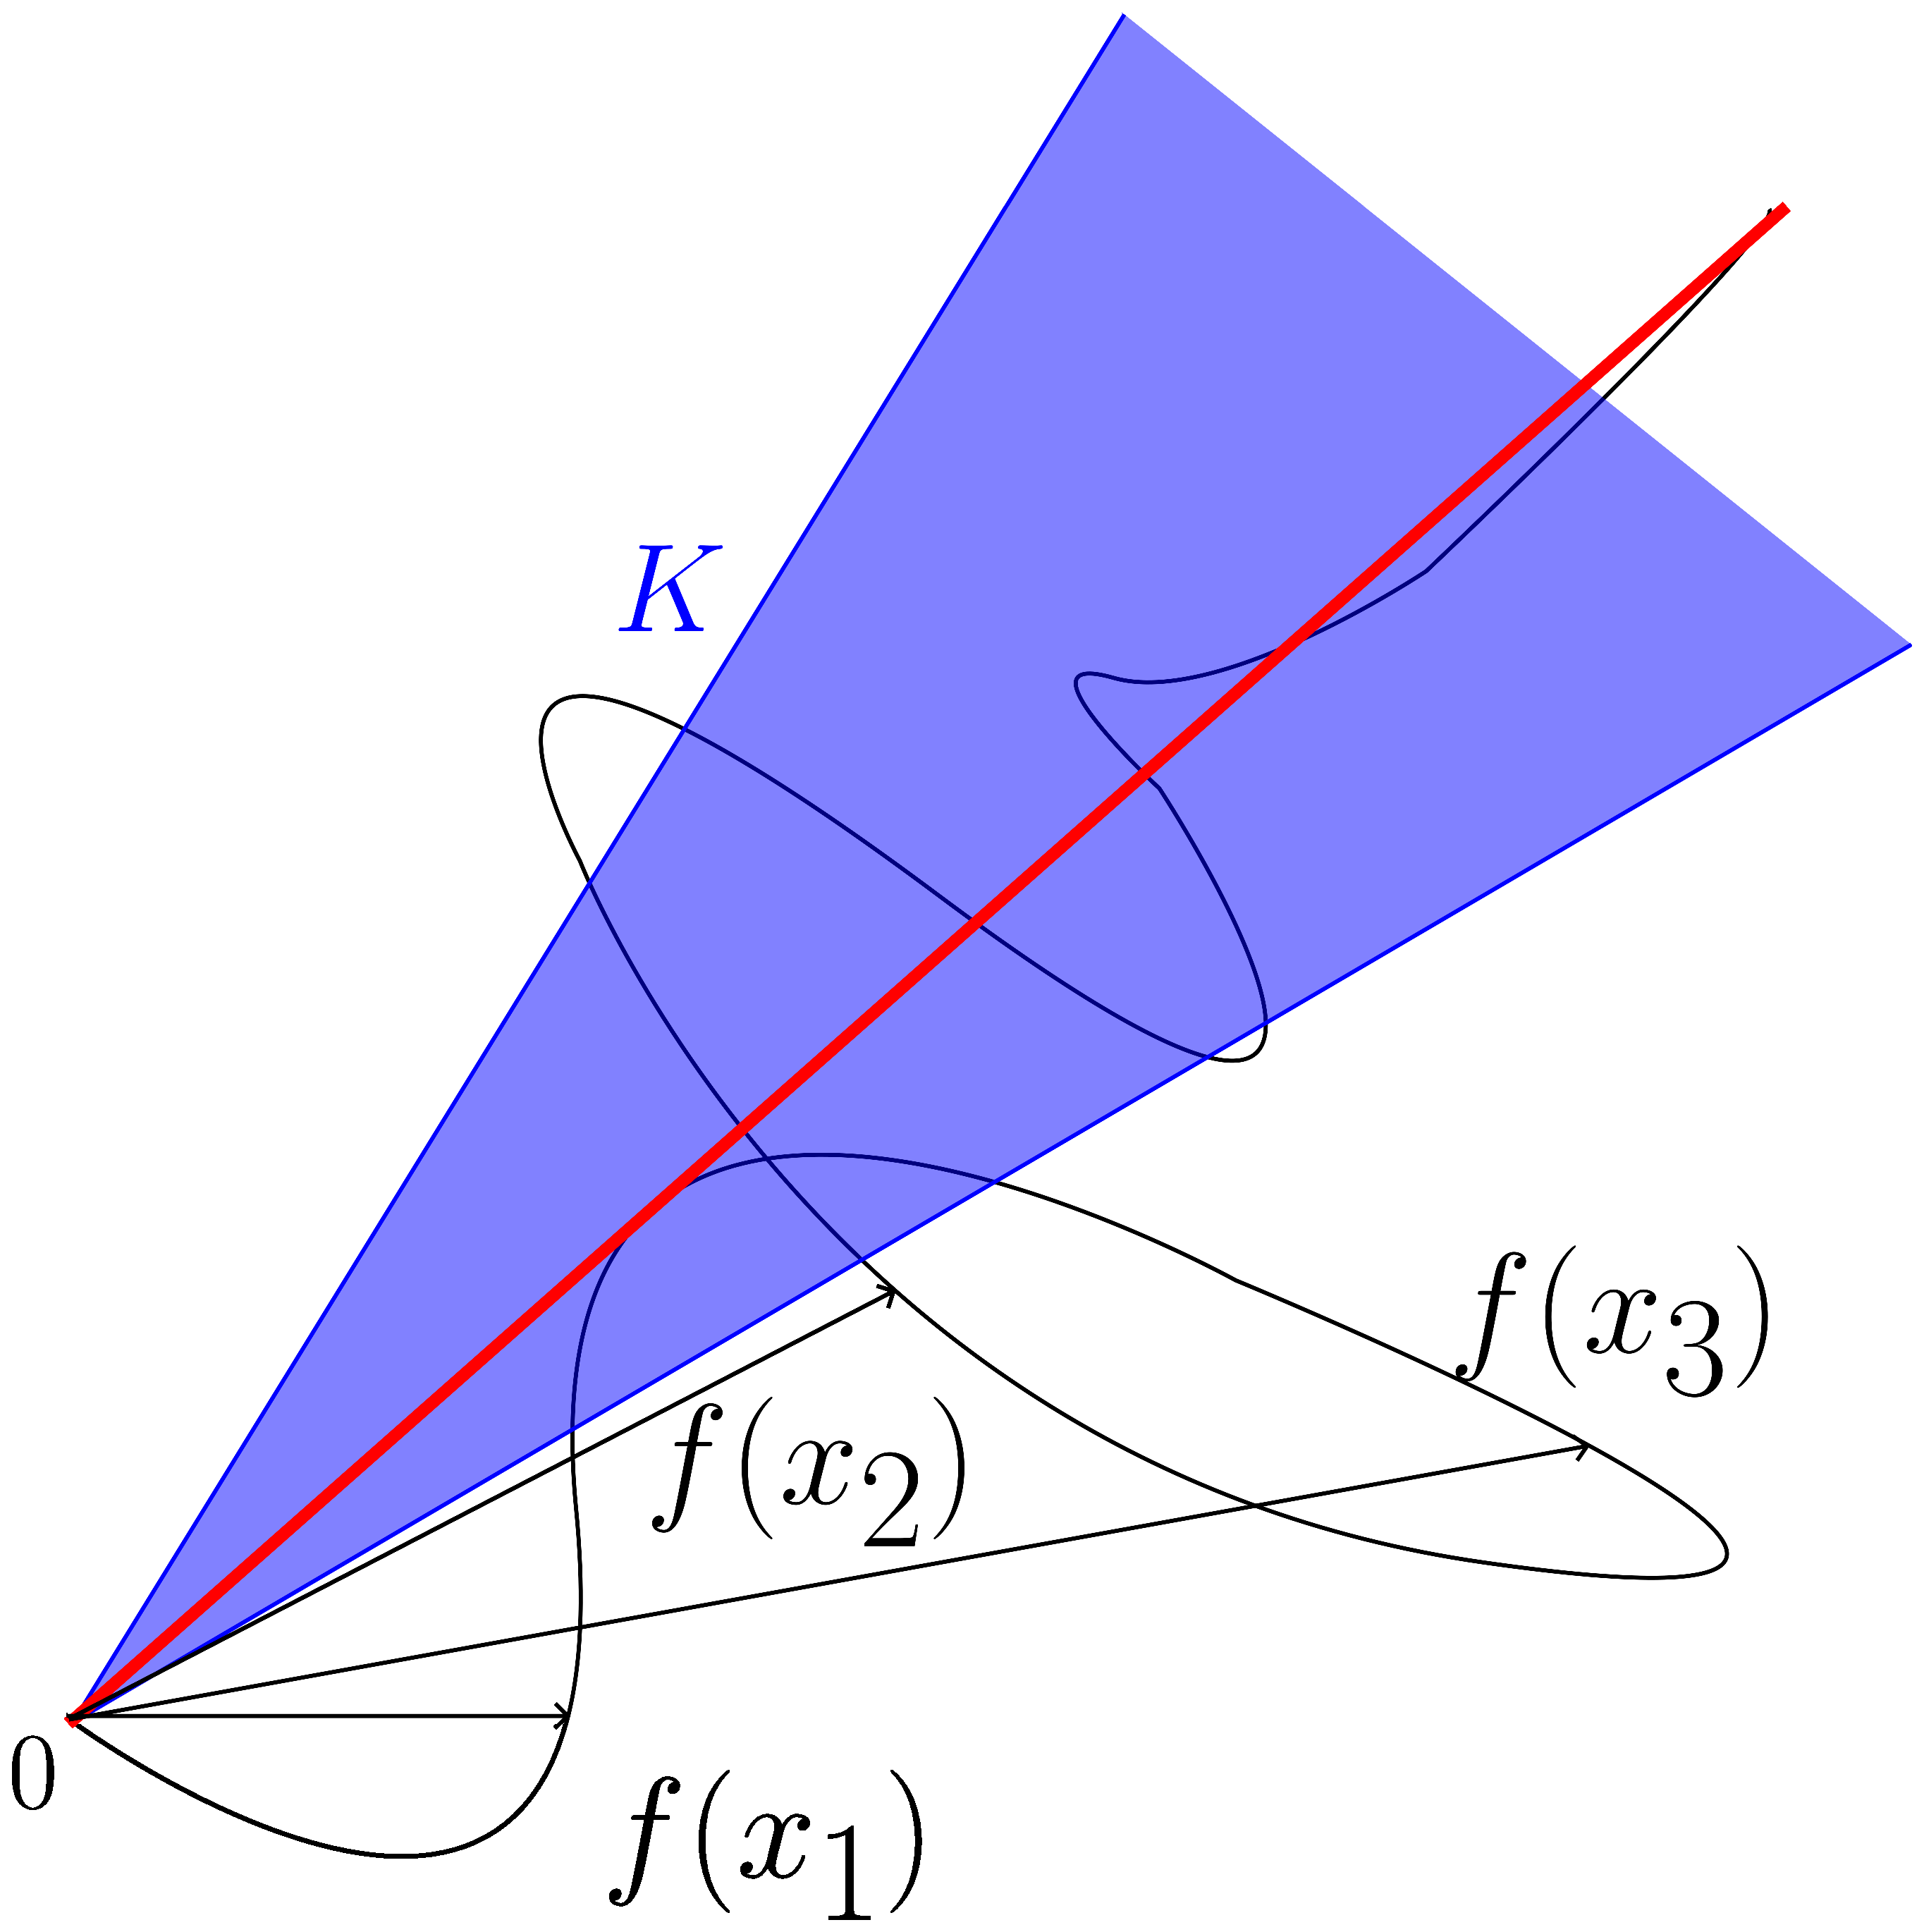
\includegraphics[width=0.9\columnwidth]{figures/eps/vector_valued_functions_image.eps}
      \caption{漸近錐が順序錐 $K$ に含まれる場合}
      \label{fig:a}
  \end{minipage}
  \begin{minipage}[b]{0.49\columnwidth}
      \centering
      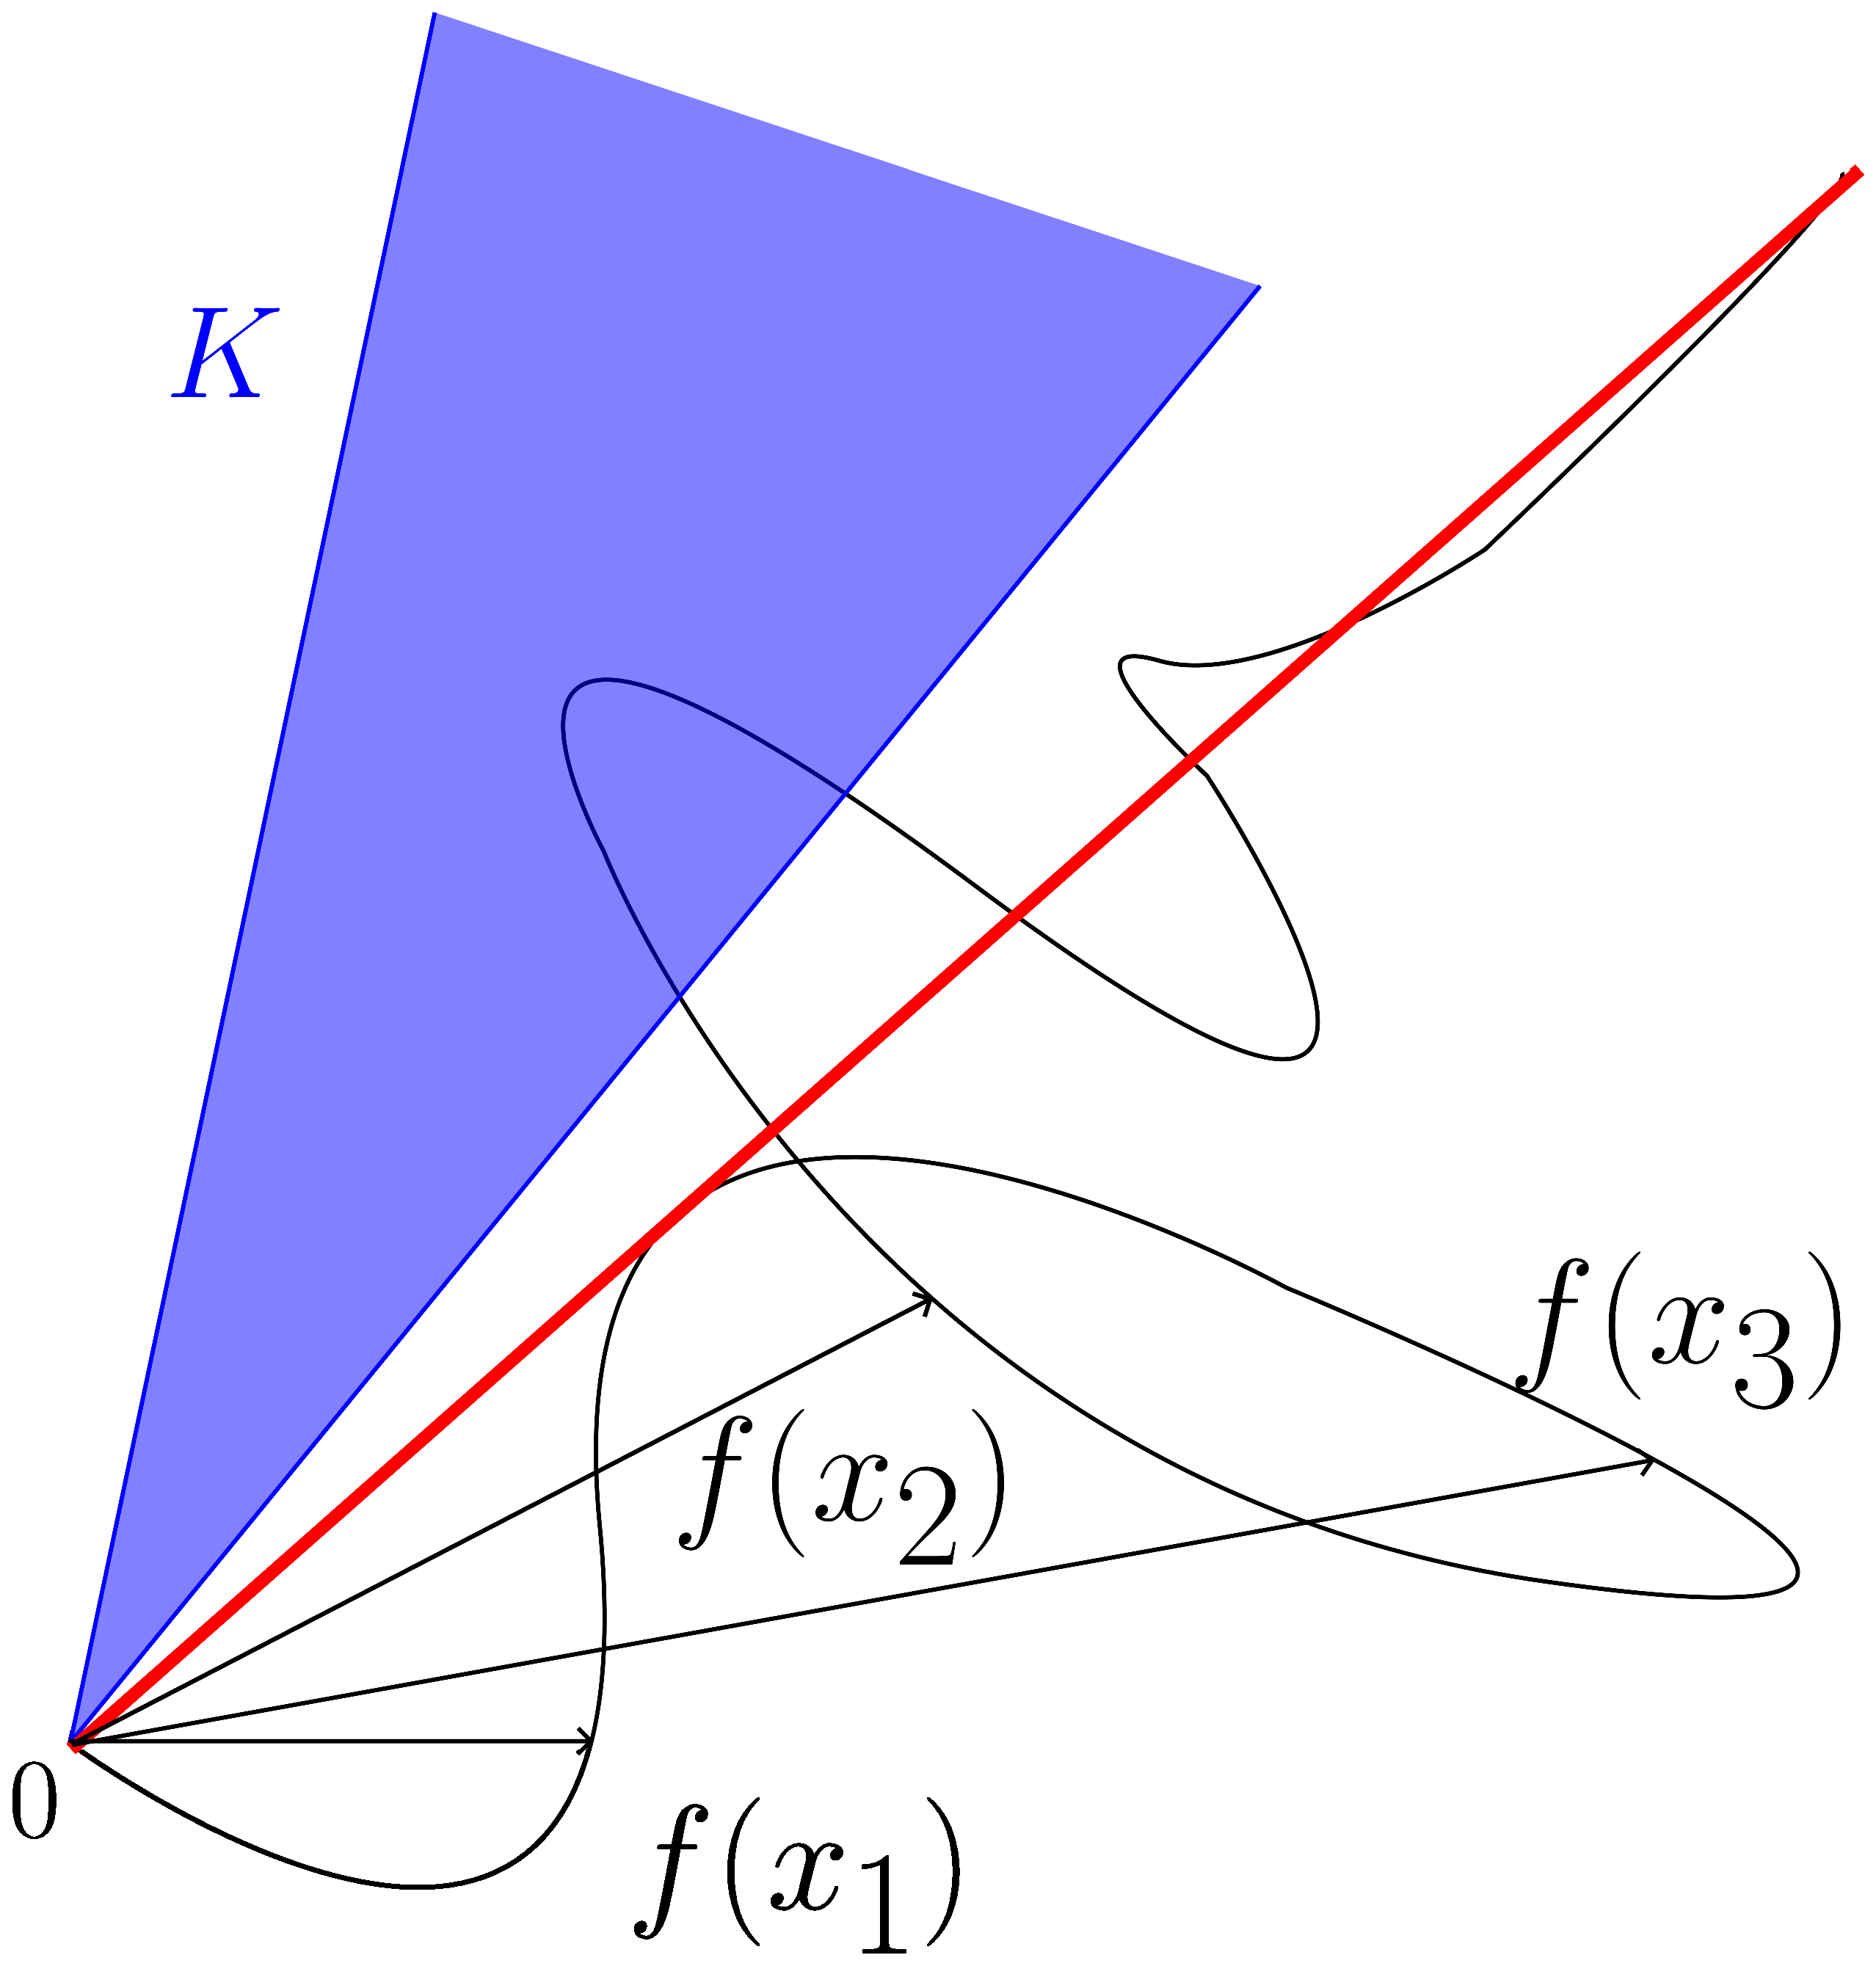
\includegraphics[width=0.9\columnwidth]{figures/eps/vector_valued_functions_image_impossible.eps}
      \caption{漸近錐が順序錐 $K$ に含まれない場合}
      \label{fig:b}
  \end{minipage}
\end{figure}

\begin{rem}
  Definition \ref{dfn1:asymptotic_function} には問題がある。それは、$(\cup_{x \in \NDemenstionalRealEuclideanSpace} \{f(x)\})_{\infty}$ が線形になるかどうかわからないことである。
\end{rem}

\begin{lem}
  Let $\VectorValuedFunction{f}{\NDemenstionalRealEuclideanSpace}{\MDemenstionalRealEuclideanSpace}$ be a vector-valued function 
  and $K$ be a closed convex cone in $\MDemenstionalRealEuclideanSpace$. Then, 
  \begin{equation}
    (\bigcup_{x \in \NDemenstionalRealEuclideanSpace} (f(x) + K))_{\infty} = (\bigcup_{x \in \NDemenstionalRealEuclideanSpace} f(x))_{\infty} + K.
  \end{equation}
\end{lem}

\begin{proof}
  ($\subset$) For any $d \in (\bigcup_{x \in \NDemenstionalRealEuclideanSpace} (f(x) + K))_{\infty}$, 
  there exist $d_k \in \bigcup_{x \in \NDemenstionalRealEuclideanSpace} (f(x) + K)$ and $t_k \rightarrow \infty$ such that
  ${t_k}^{-1}d_k \rightarrow d$ as $k \rightarrow \infty$. Let $d_k \coloneqq f(x_k) + m_k$ where $m_k \in K$. Then,
  \begin{equation}
    \frac{d_k}{t_k} = \frac{f(k_k) + m_k}{t_k} = \frac{f(x_k)}{t_k} + \frac{m_k}{t_k} 
  \end{equation}
  Since $f(x_k) \in \bigcup_{x \in \NDemenstionalRealEuclideanSpace} f(x)$ and $m_k \in K = K_{\infty}$, we obtain the inclusion.

  ($\supset$) For any $d \in (\bigcup_{x \in \NDemenstionalRealEuclideanSpace} f(x))_{\infty} + K_{\infty}$, 
  there exist $a \in (\bigcup_{x \in \NDemenstionalRealEuclideanSpace} f(x))_{\infty}$ and $m \in K_{\infty}$ such that
  $d = a + m$. By the definition of asymptotic cones, there exist $a_k \in \bigcup_{x \in \NDemenstionalRealEuclideanSpace} f(x)$ and $t_k \rightarrow \infty$ such that
  ${t_k}^{-1}a_k \rightarrow a$ as $k \rightarrow \infty$. In addition, since $K$ is asymptotically regular, for any $s_l \rightarrow \infty$, there exists $m_l \in K$ such that
  ${s_l}^{-1}m_l \rightarrow m$ as $l \rightarrow \infty$. Thus, for any $k$ sufficiently large, there exist $a_k + m_k \in (\bigcup_{x \in \NDemenstionalRealEuclideanSpace} f(x)) + K = \bigcup_{x \in \NDemenstionalRealEuclideanSpace} (f(x) + K)$ 
  and $t_k \rightarrow \infty$ such that
  \begin{equation}
    \frac{a_k + m_k}{t_k} = \frac{a_k}{t_k} + \frac{m_k}{t_k} \rightarrow a + m = d \quad\text{as}\: k \rightarrow \infty.
  \end{equation}
  Therefore, we obtain the reverse inclusion.
\end{proof}

\section{Questions}

\begin{enumerate}
  \item ベクトル値関数を考える上で、その応用として多目的最適化があるが、漸近関数をより一般化することで何が得られるか?
  \item ベクトル値にすることで sup (上限) や inf (下限) が集合として与えられるが、それに対してどのような漸近関数が考えられるか?
ベクトル値関数の共役関数は集合値関数として与えらる。そのため、漸近関数も集合値関数として定義するか、それともベクトル値関数として定義するか?
\end{enumerate}

\begin{thebibliography}{99}
  \bibitem{Auslender99}  A. Auslender. Penalty and barrier methods: A unified framework. SIAM J. Optimization, 10 (1999), 211--230.

  \bibitem{Auslender03}
  A. Auslender and M. Teboulle. Asymptotic cones and functions in optimization and variational inequalities, Springer monographs in Mathematics, Springer-Verlag, New York, 2003.

  \bibitem{BeckTeboulle12}
  A. Beck and M. Teboulle. Smoothing and First Order Methods: A Unified Framework, SIAM J. Optim, 22 (2012), 557--580.

  \bibitem{BenTalTeboulle89}
  A. Ben-Tal and M. Teboulle. A smoothing technique for nondifferentiable optimization problems. In Optimization, Fifth French-German Conference, Lecture Notes in Mathematics 1405, Springer-Verlag, New York (1989), 1--11.

  \bibitem{BorweinLewis00}
  J.M. Borwein and A.S. Lewis. Convex Analysis and Nonlinear Optimization: Theory and Examples, Springer-Verlag, New York, 2000.

  \bibitem{Lewis96}
  A.S. Lewis. Convex Analysis on the Hermitian matrices. SIAM J. Optimization, 6 (1996), 164--177.

  \bibitem{Rockafellar70}
  R.T. Rockafellar. Convex Analysis. Princeton University Press, Princeton, New Jersey, 1970.

  \bibitem{Rockafellar98}
  R.T. Rockafellar and R.J.B Wets. Variational Analysis. Springer-Verlag, New York, 1998.

  \bibitem{Seeger97}
  A. Seeger. Convex analysis of spectrally defined matrix functions. SIAM J. Optimization, 7 (1997), 679--696.

  \bibitem{Flores2024}
  F. Flores-Baz\'{a}n, R. L\'{o}pez and C. Vera. Vector Asymptotic Functions and Their Application to Multiobjective Optimization Problems. SIAM J. Optimization, 34 (2024), 1826--1851.
  
  \bibitem{Tanaka1995}
  T. Tanaka. Cone-Quasiconvexity of Vector-Valued Functions. Science Reports of the Hirosaki University, 42 (1995), 157--163.

  \bibitem{Tanaka1996}
  T. Tanaka. Approximately Efficient Solutions in Vector Optimization. J. Multi-Criteria Decision Analysis, 5 (1996), 271--278.

  \bibitem{Bot2009}
  R.I. Bo\c{t}, S.-M. Grad and G. Wanka. Duality in Vector Optimization, Springer-Verlag, Berlin-Heidelberg (2009)
\end{thebibliography}

\end{document}